\chapter{MDB and Hybrid Systems}

\section{Why models}
\begin{figure}[!h]
	\centering 
     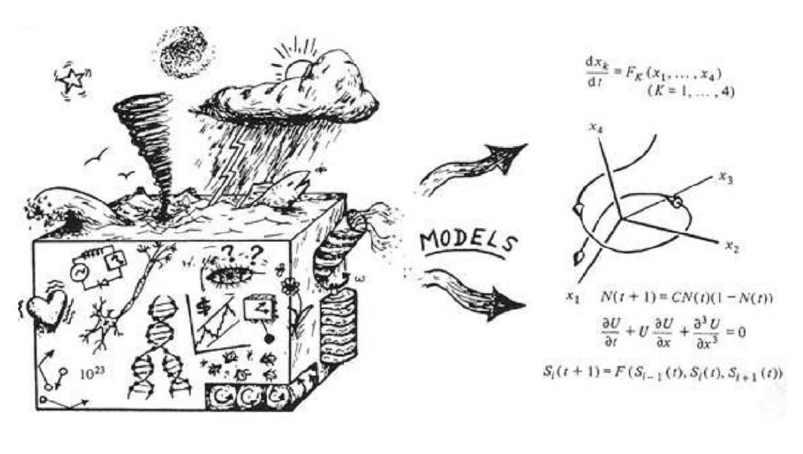
\includegraphics[width=.9\textwidth]{Figs/models.PNG} 
     \caption{Modeling} 
     \label{fig:models} 
\end{figure} 
We can define a model as a simplification of the reality (Fig.\ref{fig:models}). Models can be of any nature, \textit{mathematical models} are, typical, sets of equations, \textit{physical models} could be mock-ups aiming to provide a final picture of what the system will look like and so on.
\par Usually a model is the result of a process affected of different metrics. In a very generic perspective the first is the determination of \textit{model type}, namely which of all the possible approaches, leading to a correct result, to model our system (mathematical, graphical, textual and so on) is the most appropriate one. In practical cases this step translates in choosing the most appropriate modeling tool.
\par The second is the determination of the \textit{level of abstraction} of our model, since any system can be view as a composition of several layers one may be more interested in representing features of some of them. However, a good model has always to be connected enough to reality, indeed the risk to oversimplify may cause the model to lose meaningful information. 
\paragraph{} The previous metrics could be in turn influenced by the \textit{model purpose}. One possible scenario is when industries and organizations wants to shorten as much as possible the development time, the most natural way to accomplish that is to reuse as much as possible what they already have implemented. Reuse always implies knowledge, therefore models can be used to provide graphical and more intuitive documentations for the software or system. This is the case of UML \citep{james1999unified} and SysML\citep{sysml}, the first is a general-purpose visual modeling language that is used to specify, visualize, construct, and document the artifacts of a software system, while the latter was defined as extension of the first and provide support for the specification, analysis, design, verification, and validation of systems that include hardware, software, data, personnel, procedures, and facilities.
\paragraph{} On the other hand there could be many cases in which for a certain application domain, aerospace for instance, fully test the final product before using it's an high costly process. More, sometimes reproducing all the possible testing cases could be either too difficult or too dangerous, just think to nuclear applications. Hence, for all of these reasons, systems models could be used to simulate behavior, perform tests and verify compliance against the design. The methodology considering the model as the primary artifact for simulating the system behavior and verify properties on the behavior is called \textit{Model Based Design}.

\section{Model Based Design}

\subsection{Basis elements}

In a traditional development, usually a system engineer defines the overall system specification and presents it as a design document to software engineers, who will have the task of implementing those ideas into a fully working solution. However, the main problem with this approach is the fact that in most cases the ideas presented by the system engineer via the specification document may widely differ to the implemented software. Even the most detailed and diligently prepared type of documentation may not always guarantee that the design document generated by the system engineers would be fully understood and interpreted correctly by the implementing software programmers. The Model Based Design (MBD) approach enables behavioral modeling based on a mathematical formalism and executable semantics, and it's the reference approach for the analysis of the system, its verication by simulation, the documentation of the design and the automatic generation of a code implementation (Fig. \ref{fig:elMBD}). 

\begin{figure}[!h]
	\centering 
     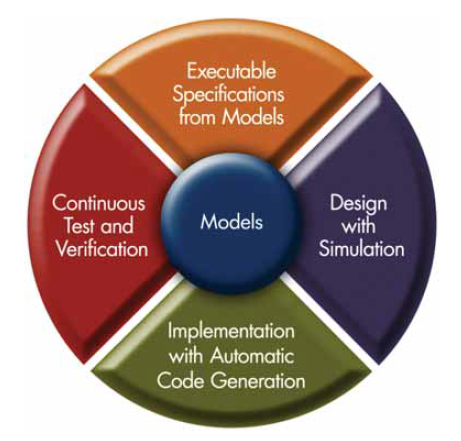
\includegraphics[width=.5\textwidth]{Figs/elementsMBD.PNG} 
     \caption{Elements of MBD} 
     \label{fig:elMBD} 
\end{figure} 

\subsection{Automatic Code Generation}

In classical development models the implementation phase follows the design, at this stage the developers will generate suitable software code in a selected language to implement the system. If the system definitions are not clear enough, the programmers would refer to system designer for clarification, but, despite these clarifications, there's still the possibility that the developed system may be different from the one that system designers had in mind. Even worse, it may contain coding errors that invalidates all the tests performed during the design. Although unlikely not even the case in which programmers job is perfect and there are no coding errors could make hand-coding the preferable approach, indeed just consider that there could be always the need to perform small changes inside the source code, such changes, whether not propagated in the models, rapidly will make the implementation divergent from the design. 
\paragraph{} MBD offers the capability to greatly improve the above approach. Within such methodology models can be used as the input to an automatic code generation tool. Usually MBD tools offers a framework at least for modeling and generate code from models, those framework commonly comprise a language offering the capability to explore model features and use them for producing target specific code.

%\paragraph{} Simulink, developed by \textit{The MathWorks Inc.}, is a block diagram environment for modeling, simulating and analyzing multidomain dynamic systems such as signal processing, control and communication applications. It supports system-level design, simulation, automatic code generation, and continuous test and verification of embedded systems. Thanks to its features, it is the \textit{de-facto} standard in MBD. 

\section{Hybrid Systems}

\subsection{State Machines}
\label{ssec:statemachines}

Systems are functions that transform signals. A broad class of systems can be characterized using the concept of state and the idea that
a system evolves through a sequence of changes in state, or state transitions. Such characterizations are called state-space models.
A state-space model describes a system procedurally, giving a sequence of step-by-step operations for the evolution of a system. It shows how the input signal drives changes in state, and how the output signal is produced. 
\paragraph{} A description of a system as a function involves three entities: the set of input signals, the set of output signals, and the function itself,
\begin{center}
$F: InputSignals \rightarrow OutputSignals $
\end{center}
For a state machine, the input and output signals have the form
\begin{center}
$EventFlow: \mathbb{N}_{0} \rightarrow Symbol$
\end{center}
where $\mathbb{N}_{0}=\{0,1,2,...\}$ and $Symbol$ is an arbitrary set. The domain of these signals represents an ordering relation that does not necessarily corresponds to time, discrete or continuous. Ordering of the domain means that it is possible to say whether one event occurs before or after another one, but without the knowledge of how much time elapses between these events.
\paragraph{} We can define \textit{state machine} that entity that constructs the output signal one symbol at a time by observing the input signal one symbol at a time. Specifically
\begin{center}
$StateMachine = (States, Inputs, Outputs, update, initialState)$
\end{center}
where $States$, $Inputs$, $Outputs$ are sets, $update$ is a function, and $initialState \in States$. The
meaning of these names is:
\begin{description}
	\item[States] is the set space
	\item[Inputs] is the input alphabet
    \item[Outputs] is the outputs alphabet
    \item[initialState] is the initial state $\in States$
    \item[update]: $States \times Inputs \rightarrow States \times Outputs$ is the update function
\end{description} 
The update function makes possible for the state machine to construct, step by step, the output signal by observing the input signal. In particular, if $x(n) \in States$ is the current state at step $n$, and $u(n) \in Inputs$ is the current input symbol, then current output symbol and the next state are given by the following
\begin{center}
$(x(n+1),y(n)) = update(x(n),u(n))$
\end{center}
The above could be decomposed in two different functions, one for new state and one for output 
\begin{flalign}
\label{form:nextstate}
&x(n+1)=nextstate(x(n),u(n)) \\
\label{form:output}
&y(n)=output(x(n),u(n))
\end{flalign}
where
\begin{flalign*}
&nextstate:  States \times Inputs \rightarrow States \\
&output:  States \times Inputs \rightarrow  Outputs
\end{flalign*}

\subsection{Time-Based Model}
\label{ssec:timemodel}

The previous section defines input and output signals of a state machine as a collection of \textit{events}. These events are generated in a domain which, usually, does not have a relation with a time set but, rather, represents just an ordered set. If we require events to happen at time instants that are multiple of a certain time quantity $\delta$ we have that
\begin{center}
$t\_e_{i}-t\_e_{j}=\alpha\cdot\delta,\quad i>j, \alpha \in \mathbb{Z}_{+}\quad \forall i,j \in \mathbb{N}_{0}$
\end{center}
where $t\_e_{i}$ and $t\_e_{j}$ are the time instant in which occur events $e_{i}$ and $e_{j}$. Under this assumption the state machine becomes a \textit{time-based model}, i.e. it reacts at all times in a base $T$.
\paragraph{} Another specialization of could be achieved by imposing, as further assumption, that state, input and output spaces be numeric sets
\begin{center}
$States=\mathbb{R}^{N},\quad Inputs=\mathbb{R}^{M},\quad Outputs=\mathbb{R}^{K}$
\end{center}
Combining the previous two assumptions we can define a \textit{discrete-time system}, and the index $n$ in (\ref{form:nextstate}) and (\ref{form:output}) is called \textit{time index}. Finally, we require that 
\begin{center}
$u(n) \in \mathbb{R}^{M}$ and $y(n) \in \mathbb{R}^{K} \quad \forall n \in T$
\end{center}
Therefore we disallow the capability, proper of state machines, to handle special "\textit{do nothing}" input called \textit{absent}. 

\subsection{LTI System}
\label{ssec:ltisys}

In discrete-time systems the time base $T \equiv \mathbb{Z}_{+}$, a definition of continuous-time system could be achieved if we relax $T$ to $\mathbb{R}_{0^{+}}$. This last category of systems shares many mathematical properties with its discrete-time version, but they can no longer be view as state machines since inputs, outputs, and state transitions do not occur at discrete instances.

\noindent
\\
Formally, a representation of a continuous time system is given, $\forall t \in \mathbb{R}_{0^{+}} $, by
\begin{flalign*}
&\dot{x}(t)=nextstate(x(t),u(t)) \\
&y(t)=output(x(t),u(t))
\end{flalign*}
The system is defined as \textit{linear} if functions $nextstate$ and $output$ are linear. It is also said \textit{time invariant} if both do not change over time. As result a system holding these two properties is said Linear Time Invariant (LTI). An interesting property of those system is that they can be represented in a compact matrix-based form. The $nextstate$ function is a $N\times (N+M)$ matrix, while the $output$ is a $K\times (N+M)$ matrix. If we partition both in two sub-matrix, the first of each comprising the first $N$ columns we get
\begin{flalign*}
\dot{x}(t)=Ax(t)+Bu(t) \\
y(t)=Cx(t)+Du(t)
\end{flalign*}
where $A \in \mathbb{R}^{N\times N}, B \in \mathbb{R}^{N\times M}, C \in \mathbb{R}^{K\times N}$ and $D \in \mathbb{R}^{K\times M}$.
\par The major difference between discrete and continuous system is that the new state is represented with the derivative of the current state instead of a function of current input and state. The motivation is that the derivative, which represents the trend of a function, better depicts the continuous evolution of the system rather than express it as a value at the successive time index.


\subsection{Mixed Models}

Sections \ref{ssec:statemachines} and \ref{ssec:timemodel} provided definitions of state machines and time-based model, trying to qualify the latter by imposing some constraint on the, more general, model of the first. In \ref{ssec:ltisys} such link was definitively broken due to the relaxation of the time to a continuous set. 
\paragraph{} In general, the two different models are used as alternative views of the same system. Even for simpler cases of discrete-time systems, which, though different from the continuous time, keep a precise mapping relationship between time and discrete time, retrieve the state machine relative to the time model is not straightforward. The reason is that operations of state machines normally acts according to a logic clear and understandable in response to situations or events that arise from the outside, such as pressing of buttons, the attainment of steady state conditions and so on.
\paragraph{} In order to get state machine models to coexist with time-based models, we need to interpret state transitions on the time line used for the time-based portion of the system, be it continuous time or discrete time. The resulting models are called hybrid systems. A hybrid system combines time-based signals with sequences of events. The time-
based signals are of the form $x : T \rightarrow R$ where $R$ is some range (such as $\mathbb{R}$ or $\mathbb{C}$), and $T$ is the time domain, discrete or continuous. In \ref{ssec:statemachines} we defined the event signals as 
\begin{center}
$u: \mathbb{N}_{0} \rightarrow Symbols$
\end{center}
for a hybrid system, however, these have to share a common time base with the time-based signals, so they must be in the form 
\begin{center}
$u: T \rightarrow Symbols$
\end{center} Thus, events occur in time. Typically, for most $t \in T$, $u(t) = absent$, meaning that the state machine does not perform any action.

\subsection{Formal Model}

The general structure of an hybrid system is shown in figure \ref{fig:hsstruct}.
\begin{figure}[!ht]
	\centering 
     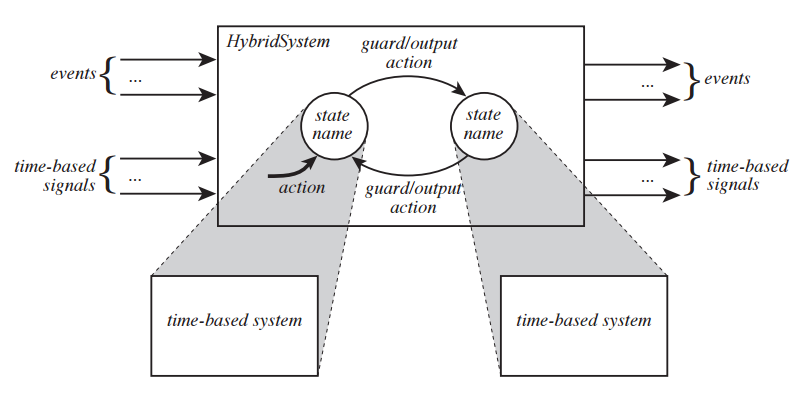
\includegraphics[width=\textwidth]{Figs/HS.PNG} 
     \caption{Hybrid System Structure} 
     \label{fig:hsstruct} 
\end{figure} 
\paragraph{} As previously mentioned, inputs and outputs may include either asynchronous events and time-based signals. In addition, each state of the state machine is associated with a time-based system, which is usually named \textit{refinement} of the state. The refinement represents the time-based behavior of the hybrid system while the internal machine is in the relative state. In order to prevent mess in the notation, those state referring to the state machine are usually called \textit{modes} while with \textit{states} are referred those of the refinements. Such notation strengthen the concept of a systems which alternates different time-based behaviors depending on the operating mode. Summarizing, for \textit{state} of an hybrid system is meant the pair $(m(t),s(t))$ where $s$ is the state of the time-based refinement system associated with mode $m$.

\noindent 
\\
A formal model for an hybrid system could be defined similarly to the one in \ref{ssec:statemachines}, indeed
\begin{center}
$HybridSystem = (States, Inputs, Outputs, TransitionStructure, initialState)$
\end{center}
where $States, Inputs$ and $Outputs$ are sets, $initialState \in States$ is the initial state and $TransitionStructure$ is the evolving law of the system in time $t \in T$, from now on we assume $T \equiv \mathbb{R}_{+}$.

\noindent
\\
$States = Modes \times RefinementStates$ represents the state space containing pairs \textit{mode}, \textit{refinementState} as previously mentioned. The set of possible modes is finite, while no constraint are on the refinement state set. 

\noindent
\\
$Inputs = InEvents \times TimeInputs$ corresponds to the set of input symbols. $InEvents$ is an alphabetic set in which each symbol stands for the description of the event, it also includes the special "do nothing" input \textit{absent}. $TimeInputs$, instead, contains all the inputs to which the refinement reacts. A complete input to the hybrid system is hence the functions pair $u:\mathbb{R}_{+}\rightarrow InEvents$ and $x:\mathbb{R}_{+}\rightarrow TimeInputs$. It's useful to recall that, apart for a limited number of cases, the function relative to the events for the most of the time is set to the value \textit{absent}.

\noindent
\\
$Outputs = OutEvents \times TimeOutputs$ is the set of output symbols. In strong analogy with what already done for the $Inputs$ set, we can identify $OutEvents$ as the alphabetic set containing those symbol representing the description of the event, and $TimeOutputs$ as the one containing all possible outputs for the refinement. The entire output of the hybrid system is then the functions pair $v:\mathbb{R}_{+}\rightarrow OutEvents$ and $y:\mathbb{R}_{+}\rightarrow TimeOutputs$. Even in this case for the most of the time the function $v(t)$ is equal to $absent$.

\noindent
\\
The $TransitionStructure$ determines how a mode transition occurs and how the refinement state changes over time. The evolution of an hybrid system occurs with the alternation of two phases, one associated to the transitioning and the other to the keeping of the current mode. In general, for state machines the transition between states is regulated by the verification of a particular conditions named \textit{guards}. Such conditions consists of an event,internal or external, occurrence. For hybrid system the concept of guard is slightly extended, in particular, given the system in a mode $m$ with relative refinement in the state $s$, the guard leading to a destination mode $d$ has the form
\begin{center}
$G_{m,d}=U_{m,d} \times X_{m,d} \times S_{m,d} \subset InEvents \times TimeInputs \times RefinementStates$
\end{center}
commonly, associated to a mode transition there is an output event $v_{m,d}$ and a function \textit{action}, $A_{m,d}:RefinementStates\rightarrow RefinementStates$, which updates the value of the refinement state. The transition from mode $m$ to mode $d$ occurs at time $t$ if the triple $(u(t),x(t),s(t))\in G_{m,d}$. If it is the case, after the transition (which is considered instantaneous) the system starts operating in mode $d$ with refinement state equal to $s(t+) = A_{m,d}(s(t))$, producing the output event $v_{m,d}$. In the case no guard is satisfied at time $t$ the systems evolves in the current mode. The refinement state $s(t)$ and the time-based output $y(t)$ are then determined by the time-based input signal $x(t)$ according to equations governing
the refinement dynamics (see Sec.\ref{ssec:ltisys}). The alternation of the two phases discussed above can be represented as $\bigcup\limits_{i=0}^{\infty}(t_i,t_{i+1}]$, during each interval the active phase is the one who maintain constant the operation mode, while the transition phase take place at the rightmost time instant of every interval.

\subsection{Examples}

\paragraph{Timed Automata} The simplest continuous-time hybrid systems that can be analyzed is a timed finite state machine measuring passage of time, it has a very simple refinement dynamics that can be modeled with a first-order differential equation,
\begin{align*}
\dot{s}(t)=1, \quad \forall t \in T_m
\end{align*}
where $T_m \subset T$ is the subset of time during which the hybrid system is in mode $m$. Figure \ref{fig:tickgen} shows a timed automata which generates a tick at time intervals alternating between 1 and 2 seconds. Although simple such example shows all the basic features of an hybrid system, namely the alternate evolution between time-count phase and tick-phase (Fig.\ref{fig:tickgenmode}), output event signal most of the time at absent value (Fig.\ref{fig:tickgenout}) and refinement output, equal to the state in this case, as a signal resulting from a differential equation (Fig.\ref{fig:tickgenstate}).
\begin{figure}[!ht]
	\centering 
     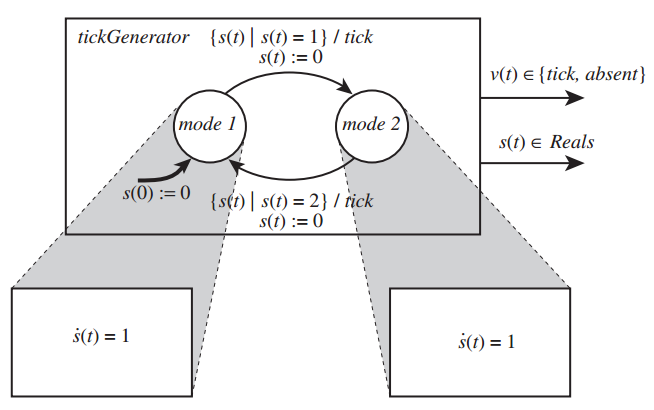
\includegraphics[width=.7\textwidth]{Figs/tickgen.PNG} 
     \caption{Hybrid System: Tick Generator} 
     \label{fig:tickgen} 
\end{figure}

\begin{figure}[!h]
  \centering
  \begin{subfigure}[b]{0.3\textwidth}
    \centering
    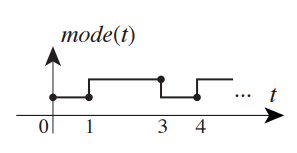
\includegraphics[width=\textwidth]{Figs/tickgenmode.PNG}
    \caption{Mode}
    \label{fig:tickgenmode}
  \end{subfigure}
  \begin{subfigure}[b]{0.3\textwidth}
    \centering
    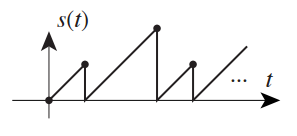
\includegraphics[width=\textwidth]{Figs/tickgenstate.PNG}
    \caption{Refinement Out}
    \label{fig:tickgenstate}
  \end{subfigure}
  \begin{subfigure}[b]{0.3\textwidth}
    \centering
    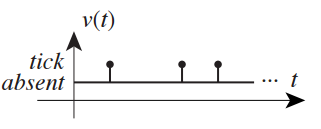
\includegraphics[width=\textwidth]{Figs/tickgenout.PNG}
    \caption{Out Event}
    \label{fig:tickgenout}
  \end{subfigure}
  \caption{Tick Generator Internals}
\end{figure}

\paragraph{Bouncing Ball} An more interesting example is an hybrid system describing the dynamics of a bouncing ball. In this case the adoption of a mixed model greatly simplifies the representation of such a system, since, being it non-linear, finding a representation only through differential equation is not easy.
\par At time $t=0$ the ball is dropped from a certain height $y(0)=h$, it freely falls, with constant velocity $\dot{y}(t) < 0\: m/s$, up to hit the ground, say at time $t1$. In that instant the \textit{bounce} events occurs and, under the assumption of inelastic collision, the ball bounces back with an inverted velocity $-a \dot{y}(t1)$, where $a \in (0,1)$. After the ball reaches a certain height it falls back  repeatedly. The model of the bouncing ball is illustrated in Figure \ref{fig:bounballhs}

\begin{figure}[!ht]
	\centering 
    \begin{subfigure}[b]{0.45\textwidth}
    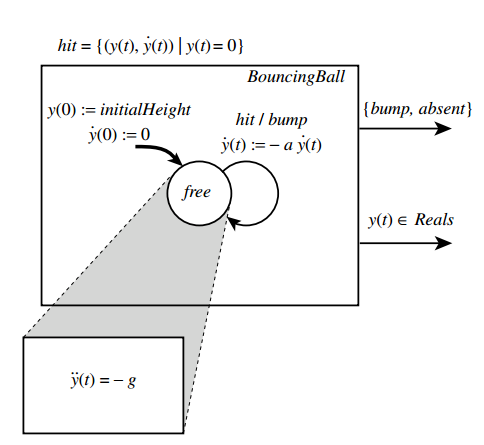
\includegraphics[width=\textwidth]{Figs/bounball.png} 
    	\caption{hybrid system} 
        \label{fig:bounballhs}
    \end{subfigure}
    \begin{subfigure}[b]{0.45\textwidth}
    	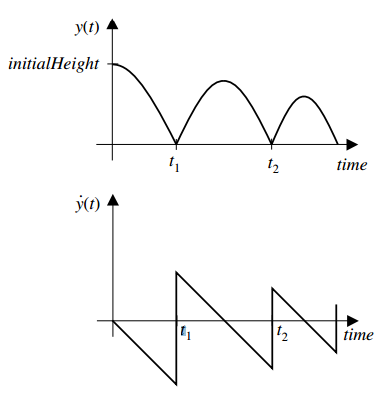
\includegraphics[width=\textwidth]{Figs/bounballout.png} 
        \caption{height and velocity} 
    	\label{fig:bounballout}
    \end{subfigure}    
     \caption{Hybrid System: Bouncing Ball} 
     \label{fig:bounball} 
\end{figure}

The \textit{hit} condition is raised whenever the height of the ball is equal to 0, namely whenever it reaches the ground. In all other time instants in order to get position and velocity of the ball is enough to double integrate the acceleration (Fig.\ref{fig:bounballout}).